\section{Surface Integrals}
% Based on Classes 31--33, Sections 17.4 and 17.5 of the lecture handouts.

\begin{problem}{Warmup: Circulation Around a Square}{vortex_square}
Let $\vv{F}(x,y) = \ang{-y,x}/(x^2 + y^2)$. Find its circulation around the square with vertices $(1,0)$, $(0,1)$, $(-1,0)$, and $(0,-1)$, traversed counterclockwise.
\end{problem}
\begin{sol}
On the first edge, $\vv{r}(t) = \ang{1 - t,t}$ for $0 \le t \le 1$. The dot product with $\vv{r}'(t) = \ang{-1,1}$ gives
\[
    \int_0^1 \frac{\dd{t}}{(1 - t)^2 + t^2}
    = \left[\arctan(2t - 1)\right]_0^1 = \frac{\pi}{2}.
\]
A quarter-turn rotates both the field and the tangent by the same angle, so every edge contributes $\pi/2$. The total is $\boxed{2\pi}$.
\end{sol}

\subsection{Parametrizing Surfaces}
\begin{definition}{Surface Parametrization}{surface_parametrization}
A parametrization of $S \subset \mathbb{R}^3$ is a vector-valued function
\[
    \vv{G}(u,v) = \ang{x(u,v),y(u,v),z(u,v)},\qquad (u,v) \in \mathcal{D},
\]
whose image is $S$. The planar region $\mathcal{D}$ is the parameter domain. For integration, choose patches that cover the surface once, allowing shared edges or seams of zero area.
\end{definition}

Polar coordinates give a planar model. The rectangle $0 \le r \le 1$, $0 \le \theta \le 2\pi$ maps onto the unit disk. A small rectangle in the parameter domain maps to an annular sector in the disk.

\begin{center}
\begin{tikzpicture}[>=Stealth,font=\small]
    % The shaded parameter cell maps to the shaded annular sector.
    \fill[blue!12] (0,0) rectangle (1.8,2.05);
    \fill[blue!35] (0.72,0.68) rectangle (1.44,1.03);
    \draw[blue!50!black] (0,0) rectangle (1.8,2.05);
    \draw[gray!55] (0.72,0) -- (0.72,2.05) (1.44,0) -- (1.44,2.05);
    \draw[gray!55] (0,0.68) -- (1.8,0.68) (0,1.03) -- (1.8,1.03);
    \draw[->] (-0.15,0) -- (2.2,0) node[right] {$r$};
    \draw[->] (0,-0.12) -- (0,2.42) node[above] {$\theta$};
    \node[left] at (0,2.05) {$2\pi$};
    \node[below] at (1.8,0) {$1$};
    \draw[->,thick] (2.35,1.05) -- node[above] {$\ang{r\cos\theta,r\sin\theta}$} (5.35,1.05);
    \begin{scope}[shift={(7.05,1.05)},scale=1.13]
        \fill[blue!12] (0,0) circle (1);
        \fill[blue!35] (120:0.4) -- (120:0.8) arc (120:180:0.8)
            -- (180:0.4) arc (180:120:0.4) -- cycle;
        \draw[gray!55] (0,0) circle (0.4) circle (0.8);
        \draw[gray!55] (0,0) -- (120:1);
        \draw[blue!50!black] (0,0) circle (1);
        \draw[->] (-1.15,0) -- (1.23,0) node[right] {$x$};
        \draw[->] (0,-1.15) -- (0,1.23) node[above] {$y$};
        \node[below right] at (1,0) {$1$};
    \end{scope}
\end{tikzpicture}
\end{center}

\newpage
\subsubsection{Cylinders, Spheres, and Graphs}

\begin{example}[Cylinder]
For the side of $x^2 + y^2 = R^2$ between $z = a$ and $z = b$, use
\[
    \vv{G}(\theta,z) = \ang{R\cos\theta,R\sin\theta,z},
    \qquad 0 \le \theta \le 2\pi,\quad a \le z \le b.
\]
Holding $z$ fixed gives a horizontal circle. Holding $\theta$ fixed gives a vertical line. A closed cylinder also requires the two disk caps, each parametrized at constant $z$ with $0 \le r \le R$.
\end{example}

\begin{example}[Sphere]
For $x^2 + y^2 + z^2 = R^2$, fix the spherical radius at $R$:
\[
    \vv{G}(\phi,\theta) = \ang{R\sin\phi\cos\theta,R\sin\phi\sin\theta,R\cos\phi},
    \qquad 0 \le \phi \le \pi,\quad 0 \le \theta \le 2\pi.
\]
The angle $\phi$ is measured from the positive $z$-axis. Holding $\phi$ fixed gives a latitude. Holding $\theta$ fixed gives a meridian. The upper hemisphere uses $0 \le \phi \le \pi/2$.
\end{example}

\begin{center}
\begin{tikzpicture}[>=Stealth,font=\small]
    % Draw coordinate curves on the cylinder and sphere.
    \begin{scope}[shift={(0,0)}]
        \fill[blue!8] (-1.2,0) -- (-1.2,2) arc (180:360:1.2 and 0.30)
            -- (1.2,0) arc (0:-180:1.2 and 0.30) -- cycle;
        \draw[gray!70] (-1.2,0) -- (-1.2,2) (1.2,0) -- (1.2,2)
            (0,2) ellipse (1.2 and 0.30);
        \draw[gray!55,dashed] (1.2,0) arc (0:180:1.2 and 0.30);
        \draw[gray!70] (-1.2,0) arc (180:360:1.2 and 0.30);
        \draw[blue!70!black,dashed] (1.2,0.96) arc (0:180:1.2 and 0.30);
        \draw[blue!70!black,thick] (-1.2,0.96) arc (180:360:1.2 and 0.30);
        \draw[red!70!black,thick] (-0.53,-0.27) -- (-0.53,1.73);
        \node[blue!70!black,right] at (1.25,0.96) {$z$ fixed};
        \node[red!70!black,below] at (-0.53,-0.29) {$\theta$ fixed};
    \end{scope}
    \begin{scope}[shift={(6.55,1.02)}]
        \filldraw[fill=blue!8,draw=gray!70] (0,0) circle (1.25);
        \draw[->,gray!70] (0,1.25) -- (0,1.58) node[above] {$z$};
        \draw[blue!70!black,dashed] (1.13,0.53) arc (0:180:1.13 and 0.25);
        \draw[blue!70!black,thick] (-1.13,0.53) arc (180:360:1.13 and 0.25);
        \draw[red!70!black,thick] (0,1.25) arc (90:270:0.62 and 1.25);
        \node[blue!70!black,right] at (1.19,0.53) {$\phi$ fixed};
        \node[red!70!black,below left] at (-0.45,-1.02) {$\theta$ fixed};
    \end{scope}
\end{tikzpicture}
\end{center}

\begin{example}[Graph of a Function]
The graph $z = h(x,y)$ over $\mathcal{D}$ has the parametrization
$\vv{G}(x,y) = \ang{x,y,h(x,y)}$. In particular,
\[
    \vv{G}(x,y) = \ang{x,y,\sqrt{R^2 - x^2 - y^2}},
    \qquad x^2 + y^2 \le R^2,
\]
parametrizes the same upper hemisphere using its projection onto the $xy$-plane.
\end{example}

\newpage
\subsection{Tangent Vectors and the Surface Area Element}
At $P = \vv{G}(u_0,v_0)$, the curves $\vv{G}(u,v_0)$ and $\vv{G}(u_0,v)$ give two tangent directions. Their derivatives at $P$ are
\[
    \vv{T}_u = \vv{G}_u(u_0,v_0),\qquad \vv{T}_v = \vv{G}_v(u_0,v_0).
\]
Their cross product $\vv{N} = \vv{G}_u \times \vv{G}_v$ is perpendicular to both. The parametrization is \textbf{regular} at $(u_0,v_0)$ when $\vv{N} \ne \vv{0}$. Then the two tangent vectors span a plane, and $\vv{N}/\lVert\vv{N}\rVert$ is a unit normal.

\begin{center}
\begin{tikzpicture}[>=Stealth,font=\small]
    % Map a parameter cell to a curved patch with two tangent directions.
    \draw[->] (0,0) -- (3.25,0) node[right] {$u$};
    \draw[->] (0,0) -- (0,2.05) node[above] {$v$};
    \filldraw[fill=blue!13,draw=blue!55] (1.0,0.62) rectangle (2.65,1.65);
    \draw[->,red!75!black,thick] (1.0,0.62) -- node[below] {$\Delta u$} (2.65,0.62);
    \draw[->,blue!70!black,thick] (1.0,0.62) -- node[left] {$\Delta v$} (1.0,1.65);
    \fill (1.0,0.62) circle (1.5pt) node[below left] {$(u_0,v_0)$};
    \draw[->,thick] (3.05,1.28) -- node[above] {$\vv{G}$} (4.55,1.28);
    \begin{scope}[shift={(6.1,0.72)}]
        \filldraw[fill=blue!8,draw=blue!40]
            (-0.65,-0.40) .. controls (0.36,-0.68) and (1.10,-0.43) .. (2.33,-0.15)
            .. controls (2.42,0.40) and (2.65,1.24) .. (2.97,1.68)
            .. controls (2.11,1.39) and (1.17,1.16) .. (0.35,1.45)
            .. controls (-0.15,1.05) and (-0.34,0.28) .. (-0.65,-0.40) -- cycle;
        \filldraw[fill=blue!21,draw=blue!45]
            (0,0) .. controls (0.55,-0.21) and (1.11,-0.08) .. (1.75,0.08)
            .. controls (1.94,0.48) and (2.02,0.87) .. (2.21,1.15)
            .. controls (1.56,1.02) and (1.17,0.82) .. (0.49,1.02)
            .. controls (0.23,0.75) and (0.16,0.33) .. (0,0) -- cycle;
        \draw[->,red!75!black,thick] (0,0) -- (1.43,-0.55) node[right] {$\vv{G}_u$};
        \draw[->,blue!70!black,thick] (0,0) -- (0.53,1.10) node[above right] {$\vv{G}_v$};
        \draw[->,green!45!black,thick] (0,0) -- (-0.62,1.63) node[above] {$\vv{N}$};
        \fill (0,0) circle (1.5pt) node[below left] {$P$};
    \end{scope}
\end{tikzpicture}
\end{center}

For small positive increments $\Delta u$ and $\Delta v$, the image of the parameter cell is approximated by the parallelogram spanned by $\vv{G}_u\Delta u$ and $\vv{G}_v\Delta v$. Its area is $\lVert\vv{G}_u \times \vv{G}_v\rVert\Delta u\Delta v$.

\begin{theorem}{Scalar Surface Integral}{scalar_surface_integral}
For a continuous scalar function $f$ on a piecewise smooth surface $S$ with a regular parametrization on the interior of $\mathcal{D}$,
\[
    \iint_S f\,\dd{S}
    = \iint_{\mathcal{D}} f(\vv{G}(u,v))\,
      \lVert\vv{G}_u \times \vv{G}_v\rVert\,\dd{u}\,\dd{v}.
\]
Here $\dd{S} = \lVert\vv{G}_u \times \vv{G}_v\rVert\,\dd{u}\,\dd{v}$. Taking $f = 1$ gives the surface area. For multiple patches, add their integrals.
\end{theorem}

A parametrization may degenerate at its parameter boundary. For example, the spherical chart collapses each edge $\phi = 0$ or $\phi = \pi$ to a pole, and the seam $\theta = 0$ coincides with $\theta = 2\pi$. These sets contribute zero area.

\newpage
\subsection{Computing Scalar Surface Integrals}

\begin{example}[Area Element for a Graph]
For $\vv{G}(x,y) = \ang{x,y,h(x,y)}$, the tangent vectors are
$\vv{G}_x = \ang{1,0,h_x}$ and $\vv{G}_y = \ang{0,1,h_y}$. Hence
\[
    \vv{G}_x \times \vv{G}_y = \ang{-h_x,-h_y,1},\qquad
    \dd{S} = \sqrt{1 + h_x^2 + h_y^2}\,\dd{x}\,\dd{y}.
\]
Substitute $z = h(x,y)$ into the integrand. For a circular projection, one can then change to polar coordinates, where $\dd{x}\,\dd{y} = r\,\dd{r}\,\dd{\theta}$.
\end{example}

\begin{problem}{Surface Area of a Sphere}{sphere_surface_area}
Find the area of $x^2 + y^2 + z^2 = R^2$ for $R > 0$.
\end{problem}
\begin{sol}
Using the spherical parametrization $\vv{G}(\phi,\theta)$ above gives
\begin{align*}
    \vv{G}_{\phi} &= R\ang{\cos\phi\cos\theta,\cos\phi\sin\theta,-\sin\phi},\\
    \vv{G}_{\theta} &= R\sin\phi\ang{-\sin\theta,\cos\theta,0},\\
    \vv{G}_{\phi} \times \vv{G}_{\theta}
        &= R^2\sin\phi\ang{\sin\phi\cos\theta,\sin\phi\sin\theta,\cos\phi}.
\end{align*}
The vector in angle brackets has unit length, so the area factor is $R^2\sin\phi$ on $0 \le \phi \le \pi$. Therefore
\[
    \operatorname{Area}(S)
    = \int_0^{2\pi}\int_0^\pi R^2\sin\phi\,\dd{\phi}\,\dd{\theta}
    = R^2(2\pi)(2) = \boxed{4\pi R^2}.
\]
\end{sol}

A spherical cell has side lengths approximately $R\,\Delta\phi$ and $R\sin\phi\,\Delta\theta$. The latitude radius $R\sin\phi$ shrinks toward either pole, which accounts for the factor $\sin\phi$.

\newpage
\begin{problem}{Gold Paint on a Paraboloid}{gold_paint_surface}
The outside of a vase is the surface $z = x^2 + y^2 + 1$ with $z \le 10$, with coordinates in inches. The paint has surface density $f(x,y,z) = z$ ounces per square inch. Set up the integral for the total amount of gold paint.
\end{problem}
\begin{sol}
The height cutoff gives $x^2 + y^2 \le 9$, so the polar radius satisfies $0 \le r \le 3$. For $h(x,y) = x^2 + y^2 + 1$,
\[
    \sqrt{1 + h_x^2 + h_y^2} = \sqrt{1 + 4x^2 + 4y^2} = \sqrt{1 + 4r^2}.
\]
The height, surface area factor, and polar Jacobian give
\[
    \boxed{M = \int_0^{2\pi}\int_0^3 (1 + r^2)\sqrt{1 + 4r^2}\,r\,\dd{r}\,\dd{\theta}}
    \qquad \text{ounces}.
\]
The same area factor follows directly from $\vv{G}(r,\theta) = \ang{r\cos\theta,r\sin\theta,1 + r^2}$, for which $\vv{G}_r \times \vv{G}_{\theta} = \ang{-2r^2\cos\theta,-2r^2\sin\theta,r}$.
\end{sol}

\begin{problem}{Center of Mass of a Hemispherical Shell}{hemisphere_centroid}
Find the center of mass of the upper half of the unit sphere with uniform surface density $\sigma > 0$. The shell consists of the curved hemisphere.
\end{problem}
\begin{sol}
Reflection across either vertical coordinate plane preserves the shell and the density. Hence $\bar{x} = \bar{y} = 0$. The mass is $M = 2\pi\sigma$, half that of the full sphere. Using $z = \cos\phi$ and $\dd{S} = \sin\phi\,\dd{\phi}\,\dd{\theta}$,
\[
    \bar{z} = \frac{1}{M}\iint_S z\sigma\,\dd{S}
    = \frac{\sigma}{2\pi\sigma}\int_0^{2\pi}\int_0^{\pi/2}
        \cos\phi\sin\phi\,\dd{\phi}\,\dd{\theta}
    = \frac{1}{2}.
\]
The center of mass is $\boxed{(0,0,1/2)}$.
\end{sol}

\newpage
\subsection{Orientation of a Surface}

\begin{definition}{Oriented Surface}{oriented_surface}
An orientation is a continuous choice of unit normal $\vv{n}$ on a smooth surface. On a connected orientable surface there are two choices. Write $-S$ for the surface with the opposite orientation.
\end{definition}

The order $\vv{G}_u \times \vv{G}_v$ induces a normal direction. Reversing the order reverses the normal, with the same length. On a cylinder or sphere, a positive dot product with an outward radial vector gives an outward normal.

\begin{problem}{Which Way Does the Normal Point?}{surface_orientation_questions}
Determine the direction of the ordered cross product for each parametrization:
\[
    \vv{G}(\theta,z) = \ang{2\cos\theta,2\sin\theta,z},\qquad
    \vv{H}(\theta,\phi) = 2\ang{\sin\phi\cos\theta,\sin\phi\sin\theta,\cos\phi}.
\]
\end{problem}
\begin{sol}
On the cylinder,
$\vv{G}_{\theta} \times \vv{G}_z = \ang{2\cos\theta,2\sin\theta,0}$, so the normal points \textbf{outward}.
On the sphere, the parameter order is $(\theta,\phi)$. Reversing the order from the sphere area calculation gives
\[
    \vv{H}_{\theta} \times \vv{H}_{\phi} = -2\sin\phi\,\vv{H}(\theta,\phi).
\]
Since $\vv{H}$ points radially outward and $\sin\phi > 0$ for $0 < \phi < \pi$, this normal points \textbf{inward}.
\end{sol}

\subsubsection{Nonorientable Surfaces}
\begin{minipage}[c]{0.65\linewidth}
A M\"obius strip joins the ends of a strip after a half twist. A normal following the centerline comes back reversed, preventing a continuous global choice. The Klein bottle is also nonorientable. Scalar integrals still use the area factor on each patch.
\end{minipage}\hfill
\begin{minipage}[c]{0.31\linewidth}
\centering
\begin{tikzpicture}[>=Stealth,font=\small,x=0.73cm]
    % Identify the vertical edges with reversed transverse direction.
    \filldraw[fill=blue!10,draw=gray!70] (0,0) rectangle (5.5,1.2);
    \draw[->,blue!70!black,thick] (0,0) -- (0,1.2);
    \draw[->,blue!70!black,thick] (5.5,1.2) -- (5.5,0);
    \draw[dashed,->,gray!80!black] (0,0.6) -- (5.5,0.6)
        node[midway,above] {centerline};
    \node[below] at (2.75,-0.04) {Glue with a half twist.};
\end{tikzpicture}
\end{minipage}

\newpage
\subsection{Flux Across an Oriented Surface}

\begin{theorem}{Surface Integral of a Vector Field}{vector_surface_integral}
The flux of a continuous vector field $\vv{F}$ through an oriented surface $S$ is
\[
    \iint_S \vv{F}\cdot\dd{\vv{S}}
    = \iint_S (\vv{F}\cdot\vv{n})\,\dd{S}
    = \iint_{\mathcal{D}}
      \vv{F}(\vv{G}(u,v))\cdot(\vv{G}_u \times \vv{G}_v)\,\dd{u}\,\dd{v},
\]
where $\dd{\vv{S}} = \vv{n}\,\dd{S}$ and the ordered cross product agrees with the chosen orientation. If it points in the opposite direction, negate it before taking the dot product.
\end{theorem}

The sign of $\vv{F}\cdot\vv{n}$ records whether the field crosses in the chosen direction or the opposite direction. A tangent field contributes zero flux. Replacing $S$ by $-S$ negates the flux and leaves scalar surface integrals unchanged.

\begin{center}
\renewcommand{\arraystretch}{1.55}
\begin{tabular}{lcc}
    & Curve $C$ & Surface $S$\\
    \hline
    Scalar & $\displaystyle\int_C f\,\dd{s}$ & $\displaystyle\iint_S f\,\dd{S}$\\
    Vector & $\displaystyle\int_C\vv{F}\cdot\dd{\vv{r}}$ (work)
           & $\displaystyle\iint_S\vv{F}\cdot\dd{\vv{S}}$ (flux)
\end{tabular}
\end{center}

\begin{example}[Power Incident on a Solar Panel]
\begin{minipage}[c]{0.67\linewidth}
A flat panel has area $A$ in square meters. The incoming sunlight has uniform intensity $\lVert\vv{F}\rVert = 800\,\mathrm{W}/\mathrm{m}^2$. Choose $\vv{n}$ pointing into the panel and let $\alpha$ be the angle between $\vv{F}$ and $\vv{n}$ on the illuminated side. The incident power is
\[
    P = \iint_S \vv{F}\cdot\vv{n}\,\dd{S} = \boxed{800A\cos\alpha\ \mathrm{W}}.
\]
At normal incidence $P = 800A\,\mathrm{W}$. The electrical output also depends on the panel's conversion efficiency.
\end{minipage}\hfill
\begin{minipage}[c]{0.29\linewidth}
\centering
\begin{tikzpicture}[>=Stealth,font=\small,scale=0.8]
    % Both vectors point toward the same patch of the panel.
    \filldraw[fill=blue!12,draw=blue!70!black] (-1.28,-0.40) -- (0.90,-0.40)
        -- (1.35,0.40) -- (-0.83,0.40) -- cycle;
    \draw[->,orange!85!black,thick] (-1.2,2.2) node[above] {$\vv{F}$} -- (0,0);
    \draw[->,green!45!black,thick] (0,2.1) node[above] {$\vv{n}$} -- (0,0);
    \draw[gray!85] (90:0.92) arc (90:118.6:0.92);
    \node[above] at (104:1.07) {$\alpha$};
    \node[below right] at (0.90,-0.40) {$S$};
\end{tikzpicture}
\end{minipage}
\end{example}

% Based on Class 33: vector surface integrals and Faraday's law.
\newpage
\subsection{Regular Parametrizations and Flux Formulas}

The Class 33 warmup is the hemispherical-shell centroid already computed in Problem~\ref{prob:hemisphere_centroid}: $\boxed{(\bar{x},\bar{y},\bar{z}) = (0,0,1/2)}$.
It uses surface density and $\dd{S}$, rather than volume density and $\dd{V}$.

\begin{definition}{Regular Parametrization}{regular_surface}
A differentiable parametrization $\vv{G}(u,v)$ is regular at $(u_0,v_0)$ if
\[
    \vv{G}_u(u_0,v_0) \times \vv{G}_v(u_0,v_0) \ne \vv{0}.
\]
Then the tangent vectors span a tangent plane and determine a unit normal.
Use patches regular in their interiors; seams or poles on patch boundaries may have zero area.
\end{definition}

For a graph $z = h(x,y)$, use $\vv{G}(x,y) = \ang{x,y,h(x,y)}$. Then
\[
    \vv{G}_x \times \vv{G}_y = \ang{-h_x,-h_y,1},\qquad
    \dd{S} = \sqrt{1 + h_x^2 + h_y^2}\,\dd{A}.
\]
For $\vv{F} = \ang{P,Q,R}$ and the \textbf{upward} orientation,
\[
    \boxed{\iint_S \vv{F}\cdot\dd{\vv{S}}
    = \iint_{\mathcal{D}}\left[-P(x,y,h)h_x - Q(x,y,h)h_y + R(x,y,h)\right]\dd{A}.}
\]
Negate this formula for the downward orientation. The cross product already includes the area factor; do not multiply by its magnitude a second time.

\textbf{A reliable setup.}
Choose a parametrization and its parameter domain. Compute the ordered cross product, check its direction against the required orientation, substitute the surface into the field, and take the dot product. Integrate over the parameter domain only after these steps.

Reversing the orientation negates the flux. A scalar surface integral instead uses the magnitude of the cross product and is unchanged by orientation.

\newpage
\subsection{Flux Through a Paraboloid}

\begin{problem}{Upward Flux of a Radial Field}{paraboloid_flux}
Let $S$ be the portion of $z = x^2 + y^2$ below $z = 4$, oriented upward.
For $\vv{F}(x,y,z) = \ang{x,y,z}$, predict the sign of the flux and evaluate it.
\end{problem}
\begin{sol}
The projection is $\mathcal{D}: x^2 + y^2 \le 4$. For
$\vv{G}(x,y) = \ang{x,y,x^2 + y^2}$, an upward normal with its area factor is
\[
    \vv{N} = \vv{G}_x \times \vv{G}_y = \ang{-2x,-2y,1}.
\]
Before integrating, take the dot product on the surface:
\[
    \vv{F}(\vv{G}(x,y))\cdot\vv{N}
    = \ang{x,y,x^2 + y^2}\cdot\ang{-2x,-2y,1}
    = -(x^2 + y^2).
\]
It is negative except at the vertex, so the net flux is \textbf{negative}.
In polar coordinates, $x = r\cos\theta$, $y = r\sin\theta$, and $\dd{A} = r\,\dd{r}\,\dd{\theta}$. Therefore
\[
    \iint_S \vv{F}\cdot\dd{\vv{S}}
    = -\int_0^{2\pi}\!\int_0^2 r^3\,\dd{r}\,\dd{\theta}
    = -2\pi\left[\frac{r^4}{4}\right]_0^2
    = \boxed{-8\pi}.
\]
\end{sol}

\begin{center}
\begin{tikzpicture}[>=Stealth,font=\small,x=1.3cm,y=0.83cm]
    % A vertical cross-section shows the radial field and the upward normal.
    \fill[blue!8] plot[domain=-2:2,samples=65] (\x,{\x * \x}) -- cycle;
    \draw[blue!70!black,thick] plot[domain=-2:2,samples=65] (\x,{\x * \x});
    \draw[gray!65,dashed] (-2,4) -- (2,4) node[right] {$z = 4$};
    \draw[->,gray!75] (-2.35,0) -- (2.5,0) node[right] {$x$};
    \draw[->,gray!75] (0,-0.2) -- (0,4.7) node[above] {$z$};
    \draw[->,orange!85!black,very thick] (1,1) -- (1.65,1.65) node[right] {$\vv{F}$};
    \draw[->,green!40!black,very thick] (1,1) -- (-0.30,1.65) node[above left] {$\vv{N}$};
    \fill (1,1) circle (1.7pt);
    \node[below] at (0,-0.45) {Cross-section $y = 0$: $\vv{F}\cdot\vv{N} < 0$.};
\end{tikzpicture}
\end{center}

The upward normal tilts toward the axis while the field points radially away from the origin. Their obtuse angle explains the negative sign even though both vectors have positive $z$-components away from the vertex.

\newpage
\subsection{Faraday's Law of Induction}

\begin{theorem}{Faraday's Law for a Stationary Loop}{faraday}
Let $C$ be a fixed closed wire loop and $S$ a fixed oriented spanning surface with $\partial S = C$. For sufficiently smooth electric and magnetic fields,
\[
    \boxed{\mathcal{E}(t) = \oint_C \vv{E}\cdot\dd{\vv{r}}
    = -\frac{\dd{}}{\dd{t}}\iint_S \vv{B}(\vv{r},t)\cdot\dd{\vv{S}}.}
\]
The circulation $\mathcal{E}$ is the electromotive force (EMF). Orient $S$ and $C$ consistently by the right-hand rule: fingers follow $C$, and the thumb points along $\vv{n}$.
\end{theorem}

The minus sign expresses Lenz's law: the induced effect opposes the change in magnetic flux. Induction stoves and wireless chargers use this principle.

\begin{problem}{Rectangular Loop Above a Straight Wire}{faraday_rectangle}
A wire along the $x$-axis produces the magnetic field
\[
    \vv{B}(x,y,z,t) = \frac{\sin t}{y^2 + z^2}\ang{0,-z,y}.
\]
A stationary rectangular loop lies in the $xz$-plane and follows
\[
    (0,0,1) \to (0,0,2) \to (3,0,2) \to (3,0,1) \to (0,0,1).
\]
Find the matching orientation of its flat interior $R$, the induced EMF, and the times when the EMF has maximum magnitude.
\end{problem}

\begin{center}
\begin{tikzpicture}[>=Stealth,font=\small,x=1.35cm,y=0.70cm]
    % View the xz-plane from the positive y side; z is right and x is up.
    \fill[blue!10] (1,0) rectangle (2,3);
    \draw[->,gray!70] (0,0) -- (2.7,0) node[right] {$z$};
    \draw[->,orange!85!black,thick] (0,-0.3) -- (0,3.6) node[above] {$x$ (wire)};
    \draw[blue!70!black,thick] (1,0) rectangle (2,3);
    \draw[->,blue!70!black,thick] (1,0) -- (1.65,0);
    \draw[->,blue!70!black,thick] (2,0) -- (2,1.9);
    \draw[->,blue!70!black,thick] (2,3) -- (1.35,3);
    \draw[->,blue!70!black,thick] (1,3) -- (1,1.1);
    \node[below] at (1,0) {$1$};
    \node[below] at (2,0) {$2$};
    \node[left] at (0,3) {$3$};
    \node[green!40!black] at (1.5,1.55) {$\odot\ +\vv{j}$};
    \node[align=left,anchor=west] at (2.65,1.8) {Viewed from $+y$:\\$+\vv{j}$ points toward you.\\The loop is counterclockwise.};
\end{tikzpicture}
\end{center}

The first edges follow $+\vv{k}$ then $+\vv{i}$. Since $\vv{k} \times \vv{i} = \vv{j}$, choose $\boxed{\vv{n} = \vv{j}}$.

\newpage
\subsubsection{Magnetic Flux and Induced EMF}
\begin{sol}
Use $\vv{G}(z,x) = \ang{x,0,z}$ for $1 \le z \le 2$, $0 \le x \le 3$.
Then $\vv{G}_z \times \vv{G}_x = \vv{k} \times \vv{i} = \vv{j}$, so
$\dd{\vv{S}} = \vv{j}\,\dd{z}\,\dd{x}$ agrees with the loop. On $R$,
\[
    \vv{B}(x,0,z,t) = \ang{0,-\sin t/z,0},\qquad
    \vv{B}\cdot\vv{j} = -\frac{\sin t}{z}.
\]
The magnetic flux is therefore
\[
    \Phi_B(t) = \int_0^3\!\int_1^2 -\frac{\sin t}{z}\,\dd{z}\,\dd{x}
    = -3\sin t\,[\ln z]_1^2
    = -3\ln 2\,\sin t.
\]
Applying Faraday's law gives
\[
    \boxed{\oint_C \vv{E}\cdot\dd{\vv{r}} = -\Phi_B'(t) = 3\ln 2\,\cos t.}
\]
Consequently, $|\mathcal{E}(t)|$ is largest at $\boxed{t = k\pi}$, $k \in \mathbb{Z}$, with maximum magnitude $3\ln 2$.
At these times $\sin t = 0$, so the magnetic field on the loop is zero and is changing at its greatest rate in magnitude. When $|\sin t| = 1$, the flux has an extremum and the EMF is zero.
\end{sol}

\begin{center}
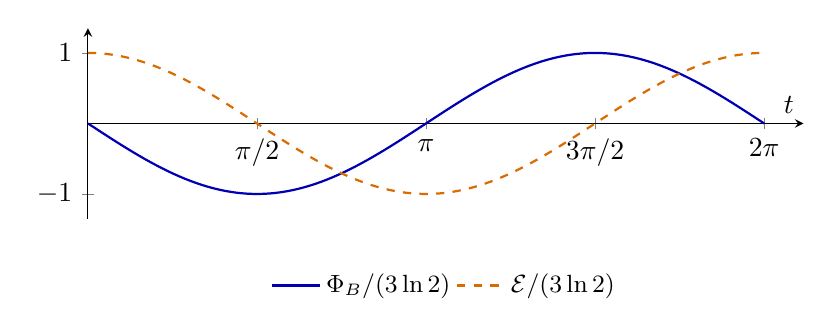
\begin{tikzpicture}
    % Normalize the flux and EMF by the common amplitude.
    \begin{axis}[
        width=0.88\linewidth,height=4.0cm,axis lines=middle,
        xmin=0,xmax=6.65,ymin=-1.35,ymax=1.35,
        xtick={0,1.5708,3.1416,4.7124,6.2832},
        xticklabels={$0$,$\pi/2$,$\pi$,$3\pi/2$,$2\pi$},
        ytick={-1,1},xlabel={$t$},samples=120,
        legend style={at={(0.5,-0.23)},anchor=north,draw=none,font=\small},
        legend columns=2,clip=false]
        \addplot[blue!70!black,thick,domain=0:6.2832] {-sin(deg(x))};
        \addlegendentry{$\Phi_B/(3\ln 2)$}
        \addplot[orange!85!black,thick,dashed,domain=0:6.2832] {cos(deg(x))};
        \addlegendentry{$\mathcal{E}/(3\ln 2)$}
    \end{axis}
\end{tikzpicture}
\end{center}

\textbf{Orientation check.} Reversing $C$ also reverses the matching surface normal. Both $\Phi_B$ and $\mathcal{E}$ change sign, while their magnitudes and the times of maximum magnitude stay the same.
